\section{Validation}
\label{sec:validation}
%
Figure ~\ref{fig:mplot} shows the $\Delta m= m^{fit}(\jpsi \mu^+ \mu^-)
- m^{em}(\jpsi \mu^+ \mu^-)$ distribution \footnote{Plotting $\Delta m$
  removes the effect of radiative corrections.   } for the $\chicone
\rightarrow J/\psi \mu^+ \mu^-$  decay mode obtained with the full
simulation and the emulator. It can be seen the agreement  is good
(allowing for a small shift). The emulator describes the core of the
distribution well but slightly underestimates the tail.
%
%
\begin{figure}[htb!]
\begin{center}
\resizebox{3.8in}{!}{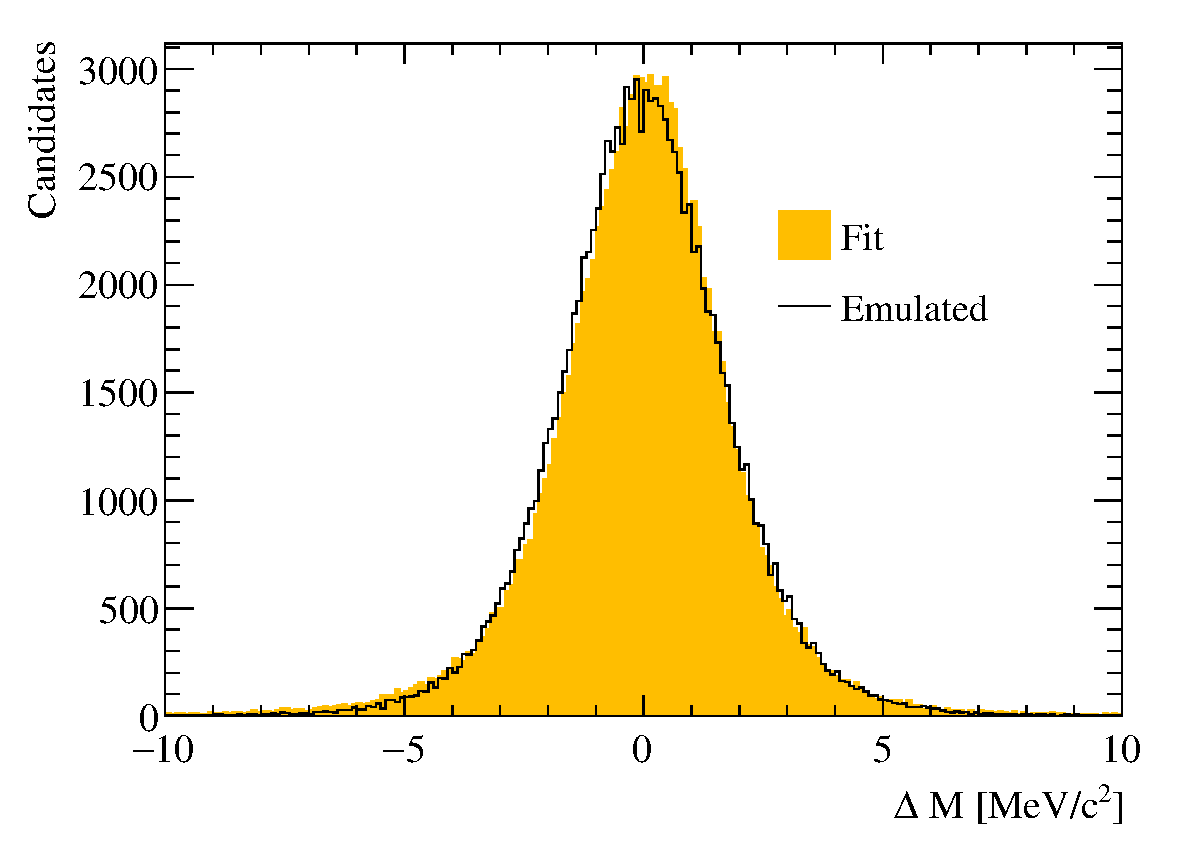
\includegraphics{figs/mplot.pdf}}
\caption{\small  Comparison of the mass resolution for the  $\chicone
\rightarrow J/\psi \mu^+ \mu^-$  decay mode with the full simulation
and the emulator. }
\label{fig:mplot}
\end{center}
\end{figure}

The quality of the emulator has been judged in two ways. First, for
the 
$\chicone \rightarrow J/\psi \mu^+ \mu^-$  decay mode the resolution
found with the full simulation and emulator using the fit model
described in Section~\ref{sec:chic} are compared as function
of the virtual photon momentum ($p_{pair}$), the candidate $\pt$ and
rapidity ($y$) in Figs.~\ref{fig:sigmappair} - \ref{fig:sigmay}. The
emulator correctly describes the trends seen with the full simulation
and the agreement is at the level of $5 \%$ or better apart from at high
$\chi_{c1}$ transverse momentum where the agreement is at the level of
$8 \%$. The disagreement at high $\pt$ is a common feature of all the
modes considered (Table \ref{tab:valid10}). This is an important
observation for the use case of using the emulator on other modes. 

%
\begin{figure}[htb!]
\begin{center}
\resizebox{3.8in}{!}{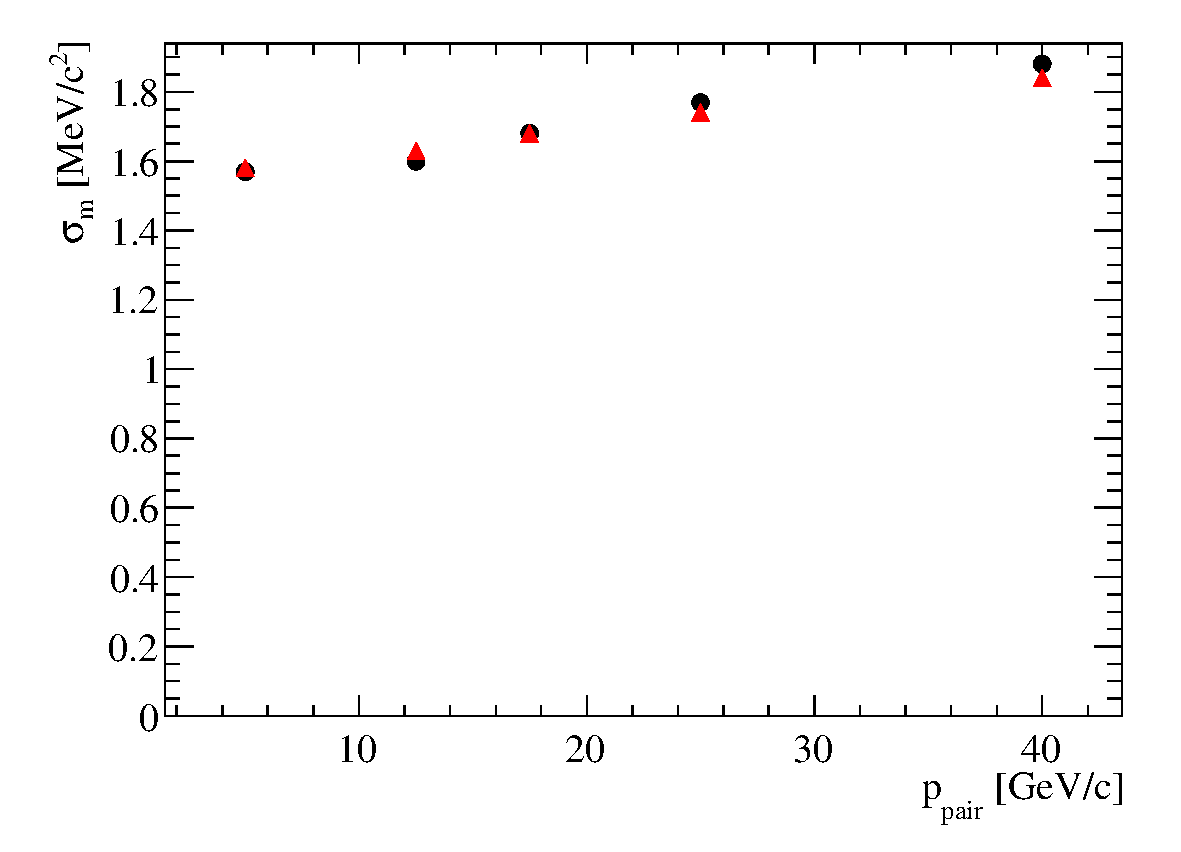
\includegraphics{figs/sigma_ppair.pdf}}
\caption{\small Mass resolution for the $\chicone \rightarrow J/\psi
  \mu^+ \mu^-$ decay sample versus $p_{pair}$. The black points are
  the results obtained with the full simulation, The red triangles are the results
  obtained with the emulator.  }
\label{fig:sigmappair}
\end{center}
\end{figure}
%
\begin{figure}[htb!]
\begin{center}
\resizebox{3.8in}{!}{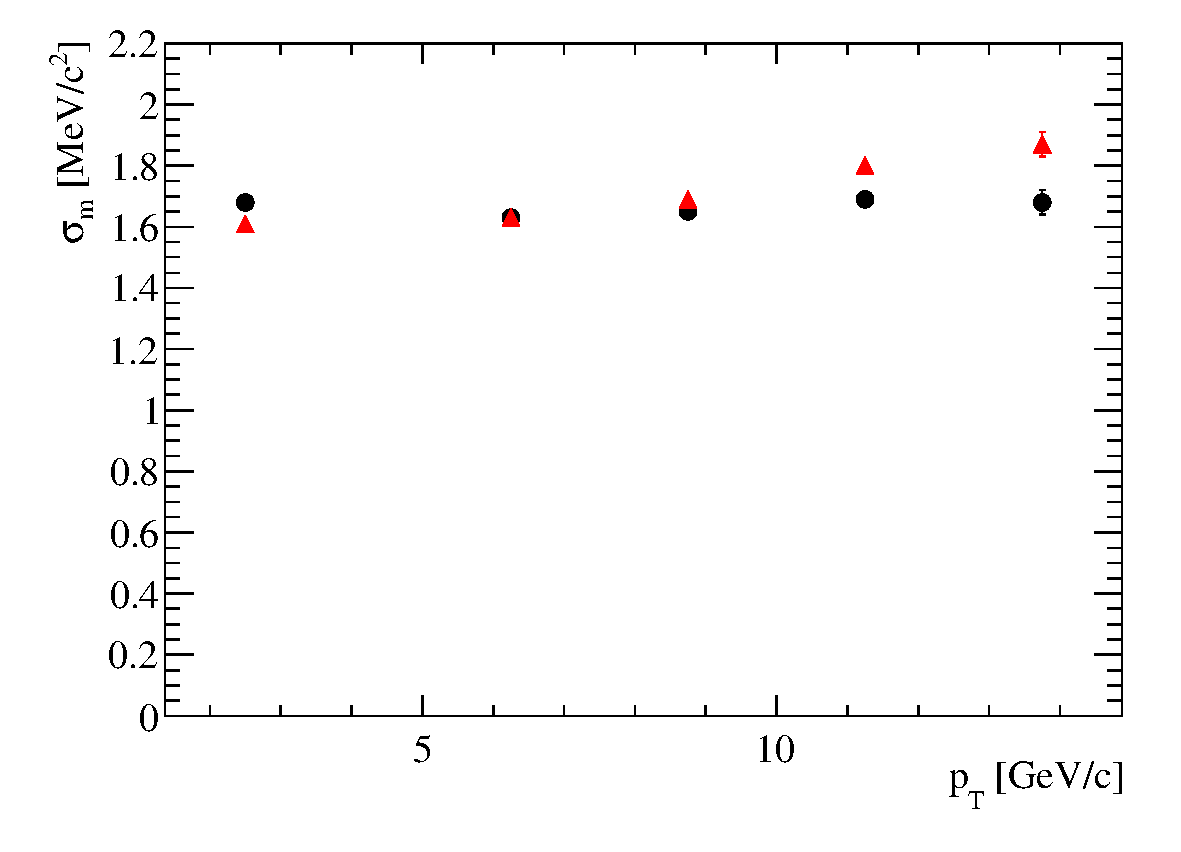
\includegraphics{figs/sigma_pt.pdf}}
\caption{\small Mass resolution for the $\chicone \rightarrow J/\psi
  \mu^+ \mu^-$ decay sample versus $\pt$.  The black points are
  the results obtained with the full simulation, The red triangles are the results
  obtained with the emulator. }
\label{fig:sigmapt}
\end{center}
\end{figure}
%
\begin{figure}[htb!]
\begin{center}
\resizebox{3.8in}{!}{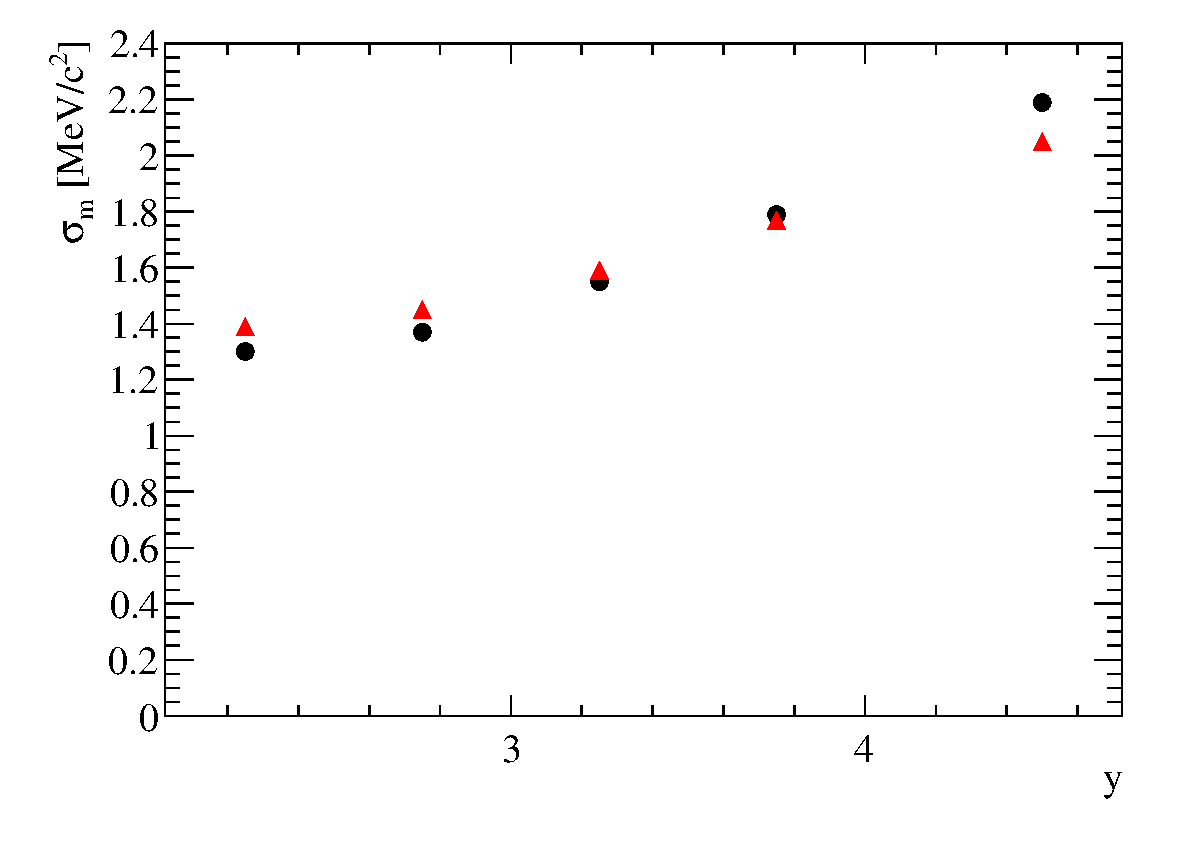
\includegraphics{figs/sigma_y.pdf}}
\caption{\small Mass resolution for the $\chicone \rightarrow J/\psi
  \mu^+ \mu^-$ decay sample versus $y$.  The black points are
  the results obtained with the full simulation, The red triangles are the results
  obtained with the emulator. }
\label{fig:sigmay}
\end{center}
\end{figure}

The second check is to compare the emulator and full simulation for
the modes $\psi(2S) \rightarrow J/\psi \pi^+ \pi^-$ and $X(3872)
\rightarrow J/\psi \pi^+ \pi^-$. The results are summarized in Table
\ref{tab:valid} and again indicate that the emulator reproduces the full
simulation at the level of $3 \%$ or better \footnote{The $\psi(2S)$
  sample is even at a different centre-of-mass energy making it a harsh test.}.

\begin{table}[htb!]
\caption{\small Comparison of the resolution found in the full
  simulation and with the emulator described in the text for several
  decay modes. }
\begin{center}
\small
\begin{tabular}{l|c|c|c|c}
Mode & Full MC Conditions & $\sigma^{fit}_m$ [$\mevcc$] &
                                                          $\sigma^{em}_m$
                                                          [$\mevcc$] &
  Ratio\\ \hline
$\chicone \rightarrow J/\psi \mu^+ \mu^-$  & 2016 & $1.66 \pm 0.01$ &
                                                                      $1.66
                                                                      \pm
                                                                      0.01$
                                                                     &
  1.0\\
$\chictwo \rightarrow J/\psi \mu^+ \mu^-$  & 2016 & $1.81 \pm 0.01$ &
                                                                      $1.83
                                                                      \pm
                                                                      0.01$
                                                                     &
  1.01\\
$\psi(2S) \rightarrow J/\psi \pi^+ \pi^-$  & 2011+12 & $2.13 \pm 0.01$
                                                        &  $2.10 \pm
                                                          0.01$ & 0.99
  \\
$X(3872) \rightarrow J/\psi \pi^+ \pi^-$  & 2016 &$2.62 \pm 0.01$ &
                                                                    $2.69
                                                                    \pm
                                                                    0.01$
                                                                     &
  1.03\\
\end{tabular}
\end{center}
\label{tab:valid}
\end{table} 



\begin{table}[htb!]
\caption{\small Comparison of the resolution found in the full
  simulation and with the emulator described in the text for several
  decay modes requring. The candidate is required to have $\pt > 10 \gevc$. }
\begin{center}
\small
\begin{tabular}{l|c|c|c|c}
Mode & Full MC Conditions & $\sigma^{fit}_m$ [$\mevcc$] &
                                                          $\sigma^{em}_m$
                                                          [$\mevcc$] &
  Ratio\\ \hline
$\chicone \rightarrow J/\psi \mu^+ \mu^-$  & 2016 & $1.70 \pm 0.02$ &
                                                                      $1.84
                                                                      \pm
                                                                      0.02$
                                                                     &
  1.08\\
$\chictwo \rightarrow J/\psi \mu^+ \mu^-$  & 2016 & $1.93 \pm 0.05$ &
                                                                      $2.13
                                                                      \pm
                                                                      0.05$
                                                                     &
  1.1\\
$\psi(2S) \rightarrow J/\psi \pi^+ \pi^-$  & 2011+12 & $2.26 \pm 0.03$
                                                        &  $2.38 \pm
                                                          0.03$ & 1.05
  \\
$X(3872) \rightarrow J/\psi \pi^+ \pi^-$  & 2016 &$2.75 \pm 0.02$ &
                                                                    $2.99
                                                                    \pm
                                                                    0.02$
                                                                     &
  1.08\\
\end{tabular}
\end{center}
\label{tab:valid10}
\end{table} 
